\documentclass[a4paper,12pt]{article}

\usepackage{cmap}
\usepackage[T2A]{fontenc}
\usepackage[utf8x]{inputenc}
\usepackage[english, russian]{babel}

\usepackage{misccorr} % в заголовках появляется точка, но при ссылке на них ее нет
\usepackage{amssymb,amsfonts,amsmath,amsthm}  
\usepackage{indentfirst}
\usepackage[usenames,dvipsnames]{color} 
\usepackage[unicode,hidelinks]{hyperref}
% \hypersetup{%
%     pdfborder = {0 0 0}
% }
\usepackage{makecell,multirow} 
\usepackage{ulem}
\usepackage{graphicx,wrapfig}
\graphicspath{{img/}}
\usepackage{geometry}
\geometry{left=2cm,right=2cm,top=3cm,bottom=3cm,bindingoffset=0cm,headheight=15pt}
\usepackage{fancyhdr} 
% \linespread{1.2} 
\frenchspacing 
\renewcommand{\labelenumii}{\theenumii)} 
% \usepackage{caption}
%%%%%%%%%%%%%%%%%%%%%%%%%%%%%%%%%%%%%%%%%%%%%%%%%%%%%%%%%%%%%%%%%%%%%%%%%%%%%%%
%%%%%%%%%%%%%%%%%%%%%%%%%%%%%%%%%%%%%%%%%%%%%%%%%%%%%%%%%%%%%%%%%%%%%%%%%%%%%%%

\def\labauthor{Автор 1, Автор 2}
\def\labauthors{\labauthor}
\def\labnumber{1}
\def\labtheme{Измерение времени жизни и диффузионной длины неосновных 
носителей заряда в полупроводниках}

%%%%%%%%%%%%%%%%%%%%%%%%%%%%%%%%%%%%%%%%%%%%%%%%%%%%%%%%%%%%%%%%%%%%%
	%применим колонтитул к стилю страницы
\pagestyle{fancy} 
	%очистим "шапку" страницы
\fancyhead{} 
	%слева сверху на четных и справа на нечетных
\fancyhead[L]{\labauthors} 
	%справа сверху на четных и слева на нечетных
\fancyhead[R]{Отчёт по лабораторной работе №\labnumber} 
	%очистим "подвал" страницы
\fancyfoot{} 
	% номер страницы в нижнем колинтуле в центре
\fancyfoot[C]{\thepage} 
\renewcommand{\phi}{\varphi}
%%%%%%%%%%%%%%%%%%%%%%%%%%%%%%%%%%%%%%%%%%%%%%%%%%%%%%%%%%%%%%%%%%%%%%%%%%%%%%%

\usepackage{float}
\usepackage[mode=buildnew]{standalone}
\usepackage{tikz} 
% \usepackage{subcaption}
\usepackage{tikz,csvsimple}
\usetikzlibrary{scopes}
\usetikzlibrary{%
     decorations.pathreplacing,%
     decorations.pathmorphing,%
    patterns,%
    calc,%
    scopes,%
    arrows,%
    % arrows.spaced,%
}
\makeatletter
\newif\if@gather@prefix 
\preto\place@tag@gather{% 
  \if@gather@prefix\iftagsleft@ 
    \kern-\gdisplaywidth@ 
    \rlap{\gather@prefix}% 
    \kern\gdisplaywidth@ 
  \fi\fi 
} 
\appto\place@tag@gather{% 
  \if@gather@prefix\iftagsleft@\else 
    \kern-\displaywidth 
    \rlap{\gather@prefix}% 
    \kern\displaywidth 
  \fi\fi 
  \global\@gather@prefixfalse 
} 
\preto\place@tag{% 
  \if@gather@prefix\iftagsleft@ 
    \kern-\gdisplaywidth@ 
    \rlap{\gather@prefix}% 
    \kern\displaywidth@ 
  \fi\fi 
} 
\appto\place@tag{% 
  \if@gather@prefix\iftagsleft@\else 
    \kern-\displaywidth 
    \rlap{\gather@prefix}% 
    \kern\displaywidth 
  \fi\fi 
  \global\@gather@prefixfalse 
} 
\newcommand*{\beforetext}[1]{% 
  \ifmeasuring@\else
  \gdef\gather@prefix{#1}% 
  \global\@gather@prefixtrue 
  \fi
} 
\makeatother

\usepackage{booktabs}
\usepackage{pgfplots, pgfplotstable}

\usepackage[outline]{contour}
\usepackage{tocloft}
\renewcommand{\cftsecleader}{\cftdotfill{\cftdotsep}} % for parts
% \renewcommand{\cftchapleader}{\cftdotfill{\cftdotsep}} % for chapters
\usepackage{pgfplots,pgfplotstable,booktabs,colortbl}
\pgfplotsset{compat=newest}
\usepackage{physics}
\usepackage{mathtools}
% \mathtoolsset{showonlyrefs=true}
\newcommand\Smat{\hat { \mathbf { S } }}
\let\tempint\int
\renewcommand{\int}{\tempint\limits}
\DeclareMathOperator{\Div}{div}
\DeclareMathOperator{\Rot}{rot}
\DeclareMathOperator{\Grad}{grad}
\DeclareMathOperator{\const}{const}
\begin{document}
\begin{titlepage}
\begin{center}

{\textsc{Нижегородский государственный университет имени Н.\,И. Лобачевского}}
\vskip 2pt \hrule \vskip 3pt
{\textsc{Радиофизический факультет}}

\vfill


{{\LARGE Отчет по лабораторной работе №\labnumber}\vskip 12pt {\Huge \bfseries \labtheme}}

	
\vspace{2cm}
{\large Работу выполнили студенты \\[-0.25em] 430 группы радиофизического факультата \\[0.5em] {\Large \bfseries \labauthor}}

% \vspace{0.5cm}
% {e-mail: sfg180@yandex.ru}

% \vspace{2cm}

\end{center}

\vfill
	
% \begin{flushright}
% 	{Выполнили студенты 430 группы\\ \labauthor}%\vskip 12pt Принял:\\ Менсов С.\,Н.}
% \end{flushright}
	
% \vfill
	
\begin{center}
	{Нижний Новгород, 3 апреля -- \today}
\end{center}

\end{titlepage}
\tableofcontents
\newpage

\section*{Введение}
\addcontentsline{toc}{section}{Введение}

Одна из особенностей полупроводниковых кристаллов состоит в том, что концентрация носителей заряда в полупроводниках сильно меняется при изменении температуры, освещении, приложении внешних электрических напряжений и т.п. Такое изменение обусловлено разрывом валентных связей кристаллической решетки полупроводника (рис. \ref{fig:figure1}).
% <img src="Время_жизни_2011_files/1240353c4f_3638373d38_2011-1.jpg" style="width:201pt;height:138pt;"/>
% <img src="Время_жизни_2011_files/1240353c4f_3638373d38_2011-2.png" style="width:194pt;height:160pt;"/>
\begin{figure}[H]
	\centering
	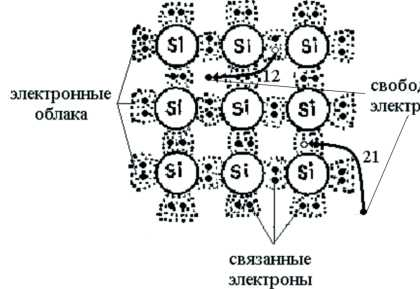
\includegraphics[]{img/1}
	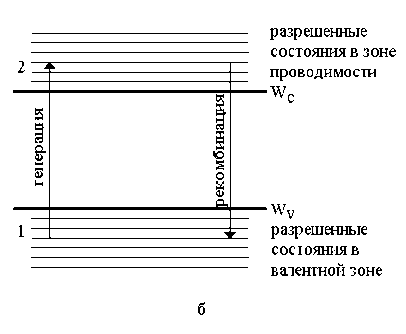
\includegraphics[]{img/2}
	\caption{Схематическое изображение кристаллической решетки кремния (а) и его зонная диаграмма (б). Стрелками указаны переходы электронов при процессах тепловой генерации из состояния 1 в состояние 2 (обозначение: 1 $\to$ 2) и обратный процесс рекомбинации (2 $\to$ 1) электронов и дырок в кристаллической решетке (а) и на зонной диаграмме (б).}
	\label{fig:figure1}
\end{figure}

Явление перехода электрона из связанного состояния в валентной зоне в зону проводимости с разрывом валентной связи называется генерацией. В процессе генерации образуется электрон в зоне проводимости и оборванная валентная связь - дырка в зоне проводимости. Обратный процесс перехода электрона в валентную зону с восстановлением валентной связи называют рекомбинацией.

Напомним, что если замкнутая макроскопическая система находится в таком состоянии, в котором для любой ее части являющейся самой по себе макроскопическим телом, макроскопические величины с большой относительной точностью равны своим средним значениям, то система находится в состоянии термодинамического равновесия [Ландау, т.5, с. 19]. Даже в условиях равновесного состояния при температурах отличных от абсолютного нуля в полупроводнике непрерывно происходит процесс теплового возбуждения электронов из валентной зоны в зону проводимости. Этот процесс уравновешивается рекомбинацией электронов из зоны проводимости и дырок из валентной зоны.

При наличии внешних воздействий на полупроводник к тепловым переходам добавляются переходы нетепловой природы, и при этом частота обратных переходов тоже изменяется. Состояние полупроводника в этих условиях является термодинамически неравновесным [Бонч-Бруевич, с. 247].

Лабораторная работа посвящена исследованию нескольких характеристик неравновесного электронно-дырочного газа -- времени жизни и диффузионной длины неосновных носителей заряда. Рекомендуется читать данное описание после описания лабораторной работы <<Измерение ширины запрещенной зоны полупроводников>>.

\section{Теоретическая часть}
\subsection{Уравнения непрерывности}

Уравнение непрерывности описывает процесс изменения плотности заряда $\rho$ в полупроводниковых структурах за счет перемещения электронов и дырок в пространстве, характеризующегося плотностью тока $\vec{j}$:

\begin{equation}
	\label{eq1}
	\frac{\partial \rho}{\partial t}=-\operatorname{div} \vec{j}
\end{equation}

Следует отметить, что кроме подвижных электронов и дырок в полупроводнике имеются неподвижные заряженные объекты - ионизованные атомы примеси, т.е. ионы доноров и акцепторов, а также заряженные дефекты кристаллической решетки. В уравнении \eqref{eq1} речь идет только о подвижных носителях заряда, в то время как для расчета электрического поля в полупроводниковых структурах следует учитывать все имеющиеся заряды.

Как отмечалось во введении, число электронов и дырок в общем случае непостоянно. Поэтому в уравнении непрерывности должны быть добавлены слагаемые, отвечающие за генерацию и рекомбинацию электронно-дырочных пар. Кроме того, поведение двух типов подвижных носителей заряда более удобно анализировать по отдельности.

\begin{gather}
	\label{eq2}
	\frac{\partial n}{\partial t}=\frac{1}{e} \Div \vec{j}_{n}+G_{n}-R_{n},\\ \nonumber
	\frac{\partial p}{\partial t}=-\frac{1}{e} \Div \vec{j}_{p}+G_{p}-R_{p}
\end{gather}

Здесь $G_n$ и $G_p$ -- скорости генерации электронов и дырок в единице объема, вызываемой внешними воздействиями, $R_n$ и $R_p$ -- скорости рекомбинации электронов и дырок.

\subsection{Генерация и рекомбинация в прямозонных и непрямозонных полупроводниках}

В процессах генерации и рекомбинации электроннодырочных пар выполняются фундаментальные физические законы - законы сохранения энергии и квазиимпульса электронов. Рассмотрим процессы, указанные на рисунке \ref{fig:figure1} во введении. Из закона сохранения энергии следует, что в процессе рекомбинации электрон выделяет избыточную энергию при переходе в валентную зону и восстановлении связанного состояния (валентной связи). Напротив, в процессе генерации электрон поглощает энергию извне, что ведет к разрыву валентной связи и переходу электрона в зону проводимости. Как в том, так и в другом случае энергия может переноситься квантом света, т.е. фотоном или квантом колебаний кристаллической решетки полупроводника - фононом. Однако не во всех типах полупроводников эти процессы равноправны. Причина этого - различные условия выполнения закона сохранения импульса при генерации и рекомбинации электронно-дырочных пар.

В прямозонных полупроводниках вершина валентной зоны и дно зоны проводимости находятся в одной точке зоны Бриллюэна (рис.  \ref{fig:figure2}б), т.е. имеют одну и туже координату по оси абсцисс (один и тот же волновой вектор). Поэтому квазиимпульс электрона, связанный с волновым вектором ($\vec{p}=\hbar \vec{k}$) при переходе почти не меняется. Значительное изменение энергии (порядка ширины запрещенной зоны) при очень малом изменении квазиимпульса возможно при испускании или поглощении кванта электромагнитного излучения, у которого, как известно, импульс мал по величине.

Напротив, в непрямозонных полупроводниках (рис.  \ref{fig:figure2}а) вершина валентной зоны и дно зоны проводимости находятся в разных точках зоны Бриллюэна. Поэтому квазиимпульс электрона сильно изменятся при межзонном переходе. Чаще всего это происходит при испускании или поглощении оптического фонона у которого квазиимпульс велик из-за большой массы атомов полупроводника, совершающих тепловые колебания. Заметим, что одновременно изменение, как энергии, так и квазиимпульса электрона при межзонном переходе происходит и при оже-рекомбинации, когда избыточная энергия и квазиимпульс передаются другому электрону или дырке. Обратным процессом оже-рекомбинации является ударная ионизация.

\begin{figure}[H]
	\centering
	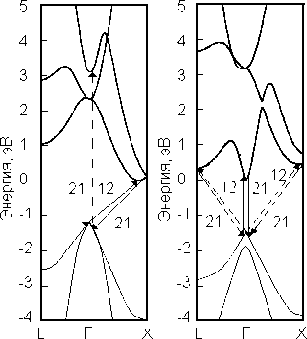
\includegraphics[]{3}
	\caption{Зонная диаграмма Si (а) и GaAs (б) полупроводников. 
Стрелками отмечены процессы генерации (1$\to$2) и рекомбинации (2$\to$1) в непрямозонных (а) и прямозонных (б) полупроводниках.    Сплошными
стрелками отмечены наиболее вероятные процессы генерации и рекомбинации, пунктиром - маловероятные. Последнее объясняется тем, что основная масса электронов и дырок имеет энергии порядка тепловых (0.037 эВ), т.е. сосредоточена около дна зоны проводимости или потолка валентной зоны. Поэтому процесс рекомбинации дырки с электроном из верхней долины маловероятен (там просто нет электронов). Если же электроны разогнать, например, в электрическом поле, так что они попадут в верхние долины, тогда рекомбинация становится возможной. Аналогично, процесс генерации электрона в верхнюю долину зоны проводимости возможен при воздействии высокоэнергичных квантов, например, ультрафиолетового диапазона}
	\label{fig:figure2}
\end{figure}
% <img src="Время_жизни_2011_files/1240353c4f_3638373d38_2011-3.png" style="width:147pt;height:162pt;"/>
% 
% рис.  2. 

Поглощение оптического излучения в полупроводнике характеризуется коэффициентом поглощения. В случае, когда энергия кванта чуть больше ширины запрещенной зоны, т.е. вблизи края фундаментального поглощения полупроводника, коэффициент поглощения определяется, как 
\begin{gather}
	\label{eq3}
	\alpha \sim\left(h\nu-W_{g}\right)^{\gamma}
\end{gather}
где $h\nu$ - энергия фотона, $W_g$ - ширина запрещенной зоны. Теоретически (в одноэлектронном приближении) $\gamma=\frac12$ для разрешенных
прямых переходов и $\gamma=2$ для непрямых переходов, которые происходят с участием фононов.

На рисунке \ref{fig:figure3} приведены экспериментальные зависимости коэффициента поглощения от энергии фотонов в Ge, Si и GaAs вблизи и выше края фундаментального поглощения. Наблюдаемое смещение кривых в сторону высоких энергий обычно связывают с температурной зависимостью ширины запрещенной зоны.


\begin{figure}[H]
	\centering
	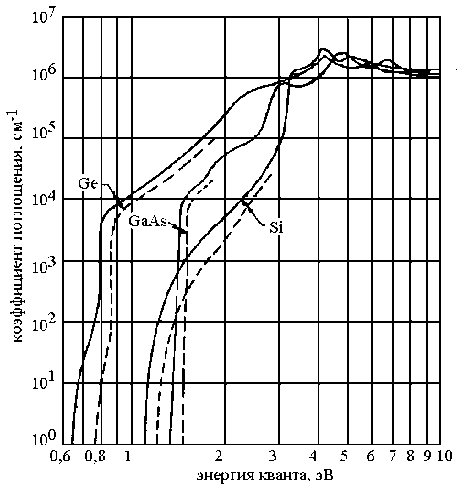
\includegraphics[]{4}
	\caption{Экспериментальные спектры оптического поглощения в чистых кристаллах Ge, Si и GaAs. Пунктиром показан коэффициент поглощения при Т = 77 К. Уменьшение коэффициента поглощения связано с изменением ширины запрещенной зоны полупроводника при охлаждении.}
	\label{fig:figure3}
\end{figure}
% <img src="Время_жизни_2011_files/1240353c4f_3638373d38_2011-4.png" style="width:222pt;height:235pt;"/>


Существенно разный ход зависимости коэффициента поглощения излучения от энергии квантов, определяемый главным образом шириной запрещенной зоны и типом перехода, позволяет создать фотодетектор, чувствительный к определенной области спектра падающего электромагнитного излучения. Поэтому в задачах детектирования излучения используются как прямозонные, так и непрямозонные полупроводники с различной шириной запрещенной зоны. В этом проявляется основное отличие от задачи излучения света, для решения которой применяются в основном прямозонные полупроводники.2

Рассмотренная выше рекомбинация типа <<зона-зона>> характерна для высококачественных полупроводниковых кристаллов. Если в полупроводнике есть дефект, например, вакансия, атом примеси или иное более сложное образование, например, комплекс точечных дефектов, то в запрещенной зоне возникают разрешенные энергетические уровни, на которые могут переходить как электроны, так и дырки (рис. \ref{fig:figure4}). При наличии дополнительных дискретных уровней в запрещенной зоне процессы генерации и рекомбинации протекают преимущественно с их участием. Это происходит потому, что при переходе электрона или дырки на уровень в запрещеннои зоне величина передаваемой носителем заряда энергии сильно уменьшается, что обуславливает большую вероятность перехода <<зона-уровень>> по сравнению с переходом <<зона-зона>>. Положение уровня в запрещенной зоне также влияет на скорость рекомбинации. Если уровень расположен вблизи середины запрещенной зоны полупроводника (так называемый глубокий уровень), то вероятность попадания на него как электрона, так и дырки примерно одинакова. Напротив, если уровень расположен вблизи валентной зоны или зоны проводимости (мелкий уровень), то вероятности попадания на такой уровень носителей разных знаков существенно различны.

Таким образом, рекомбинационные процессы при наличии глубокого уровня протекают в две стадии: сначала на глубокий уровень захватывается носитель одного знака, а затем другого. Мелкие уровни не оказывают существенного влияния на скорость рекомбинации, так как в этом случае скорость рекомбинации будет определяться меньшей из вероятностей попадания носителей на уровень. При наличии одного глубокого уровня скорость рекомбинации может быть описана на основе теории Шокли-Рида-Холла
\begin{gather}
	\label{eq4}
	R(n, p)=\frac{\sigma_{n} \sigma_{p} v_{t h}\left(p n-n_{0} p_{0}\right) N_{t}}{\sigma_{n}\left(n+\sqrt{n_{0} p_{0}} \exp \left(\frac{W_{t}-W_{F i}}{k T}\right)\right)+\sigma_{p}\left(p+\sqrt{n_{0} p_{0}} \exp \left(-\frac{W_{t}-W_{F i}}{k T}\right)\right)}
\end{gather}
где $\sigma_{n}$ и $\sigma_{p}$ -- сечения захвата электрона и дырки, $v_{th}=\sqrt{3kT/m^*}$ -- тепловая скорость носителей, $N_t$ -- концентрация ловушек, $W_t$ -- уровень ловушек, $W_{Fi}$ -- уровень Ферми в собственном полупроводнике, $k$ -- постоянная Больцмана, $Т$ -- температура полупроводника, $p$ и $n$ -- концентрации неравновесных дырок и электронов в полупроводнике, $p_0$ и $n_0$ -- концентрации равновесных носителей заряда.

Произведение сечения захвата носителей заряда, их средней скорости и концентрации представляет собой количество носителей, захватываемых на рекомбинационный уровень в единицу времени. Экспоненты в знаменателе определяют зависимость скорости рекомбинации от положения рекомбинационного уровня в запрещенной зоне полупроводника. Как и следует ожидать из физических соображений рассмотренных выше, скорость рекомбинации в равновесном состоянии равна нулю.

Скорость рекомбинации максимальна в том случае, когда рекомбинационный уровень расположен вблизи середины запрещенной зоны ($W_t\sim W_{Fi}$). Поэтому именно глубокие уровни будут наиболее эффективными рекомбинационными центрами.


\begin{figure}[H]
	\centering
	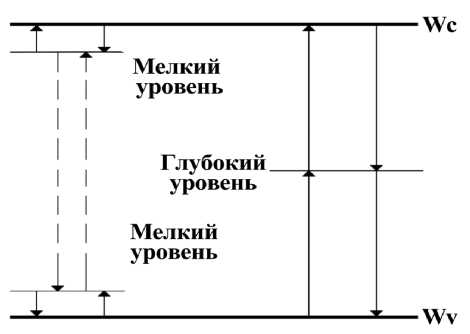
\includegraphics[]{5}
	\caption{Рекомбинационные процессы в полупроводнике с мелкими и глубоким уровнями. Пунктиром показан маловероятный процесс рекомбинации через мелкие уровни.}
	\label{fig:figure4}
\end{figure}
% <img src="Время_жизни_2011_files/1240353c4f_3638373d38_2011-5.jpg" style="width:225pt;height:160pt;"/>

Поверхность кристалла полупроводника является нарушением периодичности расположения атомов кристаллической решетки полупроводника, т.е. дефектом кристаллической решетки. Поэтому вблизи поверхности кристалла должны существовать локальные энергетические уровни в запрещенной зоне. Скорость поверхностной рекомбинации описывается формулой, аналогичной выражению \eqref{eq4}
\begin{gather}
	\label{eq5}
	R_{s}(n(0), p(0))=\frac{n(0) p(0)-n_{0} p_{0}}{n_{0}+p_{0}} \frac{s_{n} s_{p}}{\frac{s_{n} n_{0}}{n_{0}+p_{0}}+\frac{s_{p} p_{0}}{n_{0}+p_{0}}},
\end{gather}
где $s_n$ и $s_p$ - скорости поверхностной рекомбинации для электронов и дырок.

При малых уровнях инжекции, часто используют приближение <<времени жизни>>, основанное на разложении $R(n,p)$ в ряд Тейлора в линейном приближении 
\begin{gather}
	\label{eq6}
	R(n, p)=\left(\frac{\partial R}{\partial n}\right)_{p=n_{0} \atop p=p_{0}} \delta n+\left(\frac{\partial R}{\partial p}\right)_{n=n_{0} \atop p=p_{0}} \delta p
\end{gather}
Введем величины 
\begin{equation*}
	\tau_{n}=\left(\frac{\partial R}{\partial n}\right)_{n=n_{0} \atop p=p_{0}}^{-1}
	\qq{и}
	\tau_{p}=\left(\frac{\partial R}{\partial p}\right)_{n=p_{0} \atop p=p_{0}}^{-1},
\end{equation*}  имеющие размерность времени и характеризующие протяженность интервала существования неосновных носителе заряда от момента генерации до их рекомбинации.

С учетом \eqref{eq6} уравнения непрерывности можно записать в виде
\begin{gather}
	\label{eq7}
	\frac{\partial n}{\partial t}=\frac{1}{e} \Div \vec{j}_{{n}}+G_{n}-\frac{n-n_{0}}{\tau_{n}}\\
	\frac{\partial p}{\partial t}=-\frac{1}{e} \Div \vec{j}_{{p}}+G_{p}-\frac{p-p_{0}}{\tau_{p}}
\end{gather}

Скорость генерации электронно-дырочных пар, как правило, связывают с мощностью поглощенного в полупроводниковой структуре излучения
\begin{gather}
	\label{eq8}
	G=g_{0} P,
\end{gather}
где $Р$ -- мощность поглощенного излучения, a $g_0$ -- коэффициент, характеризующий свойства конкретного полупроводника.

В случае, когда к полупроводниковому кристаллу приложено большое напряжение, такое, что в некоторой области полупроводниковой структуры напряженность электрического поля имеет величину $10^5\ldots10^6\ \frac{\text{В}}{\text{см}}$ развивается лавинный пробой полупроводниковой структуры. В этом случае коэффициент генерации водят как
\begin{gather}
	\label{eq9}
	G=\alpha_{n} n v_{n}+\alpha_{p} p v_{p},
\end{gather}
 где $\alpha_n$ и $\alpha_p$ -- коэффициенты ударной ионизации для электронов и дырок, определяемые как число электронно-дырочных пар, генерируемых носителем заряда на единице пути траектории. Численные значения коэффициента ударной ионизации в зависимости от величины напряженности электрического поля приведены на рисунке \ref{eq5}.

\begin{figure}[H]
	\centering
	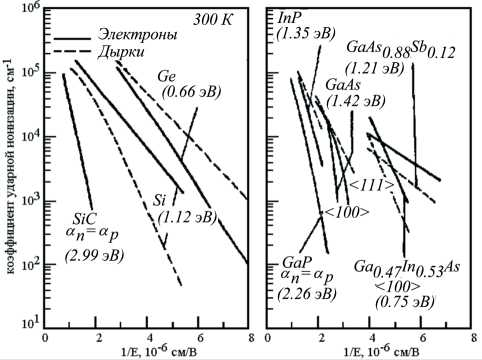
\includegraphics[]{6}
	\caption{Полевая зависимость коэффициентов ударной ионизации при Т = 300 К в Ge, Si, GaAs и некоторых других полупроводниковых соединений}
	\label{fig:figure5}
\end{figure}
% <img src="Время_жизни_2011_files/1240353c4f_3638373d38_2011-6.jpg" style="width:231pt;height:172pt;"/>



\subsection{Примеры применения уравнений непрерывности}

Релаксация фотовозбужденных носителей. Физический смысл <<времени жизни>>. Рассмотрим образец $n$-типа, освещаемый так, что свет генерирует электронно-дырочные пары равномерно по его объему. В отсутствии внешнего электрического поля и градиента концентрации дырок (образец освещается равномерно по всему объему) уравнение \eqref{eq6} для неосновных носителей - дырок имеет вид
\begin{gather}
	\label{eq9}
	\frac{\partial p}{\partial t}=G_{p}-\frac{p-p_{0}}{\tau_{p}}
\end{gather}

В стационарных условиях $\frac{\partial p}{\partial t}=0$ и
\begin{gather}
	\label{eq10}
	p_{n}=p_{n 0}+\tau_{p} G=\const
\end{gather}

Пусть в момент времени $t = 0$ освещение выключается. В последующие моменты времени $t > 0$ концентрация определяется уравнением
\begin{gather}
	\label{eq11}
	\frac{\partial p}{\partial t}=-\frac{p-p_{0}}{\tau_{p}},
\end{gather}
которое нужно решать с начальным условием \eqref{eq10}. Это решение показано на рисунке \ref{fig:figure6}.

\begin{figure}[H]
	\centering
	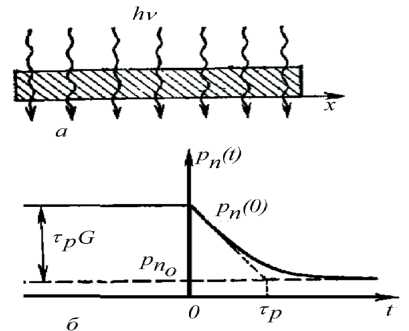
\includegraphics[]{7}
	\caption{Релаксация фотовозбужденных носителей, а) образец $n$-типа при постоянном освещении; б) зависимость концентрации неосновных носителей (дырок) от времени при выключении света в момент $t = 0$}
	\label{fig:figure6}
\end{figure}
% <img src="Время_жизни_2011_files/1240353c4f_3638373d38_2011-7.jpg" style="width:196pt;height:158pt;"/>

Из приведенного примера видно, что характерное время изменения концентрации неосновных носителей заряда равно <<времени жизни>>.

Стационарная инжекция с одной стороны образца. Диффузионная длина. Пусть избыточные носители инжектируются с одной стороны образца, например при освещении коротковолновым светом, который генерирует электронно-дырочные пары в тонком приповерхностном слое. Например, для фотонов с энергией 3.5 эВ коэффициент поглощения $10^6\ \text{см}^{-1}$, то есть интенсивность такого излучения ослабляется в $e$ раз в приповерхностном слое толщиной 10 нм, где и генерируются, в основном, избыточные носители заряда.

В стационарных условиях ($\frac{\partial p}{\partial t}=0$ ) поверхностная генерация приводит к появлению градиента концентрации неосновных носителей в приповерхностной области образца. При этом уравнение \eqref{eq5} для неосновных носителей - дырок приобретает вид
\begin{gather}
	\label{eq13}
	\frac{1}{e} \frac{\partial j_{p}}{\partial x}+\frac{p-p_{0}}{\tau_{p}}=0
\end{gather}

Поскольку отсутствует электрическое поле, то дырки перемещаются только за счет разности концентраций и существует только диффузионный ток. Он равен
\begin{gather}
	\label{eq14}
	j_{p}=-e D_{p} \frac{\partial p}{\partial x}
\end{gather}

Подставляя \eqref{eq14} в \eqref{eq13}, получим уравнение для концентрации
неосновных носителей заряда
\begin{gather}
	\label{eq15}
	D_{p} \frac{\partial^{2} p}{\partial x^{2}}-\frac{p-p_{0}}{\tau_{p}}=0
\end{gather}
с граничными условиями $p_{n}(x=0)=p_{n}(0)$ и $p_{n}(x \rightarrow \infty)=p_{n 0}$. Его решение имеет вид
\begin{gather}
	\label{eq16}
	p_{n}(x)=p_{n 0}+\left(p_{n}(0)-p_{n 0}\right) e^{-\frac{x}{L_{p}}}
\end{gather}
где $L_{p} \equiv \sqrt{D_{p} \tau_{p}}$ -- диффузионная длина неосновных носителей заряда.

\begin{figure}[H]
	\centering
	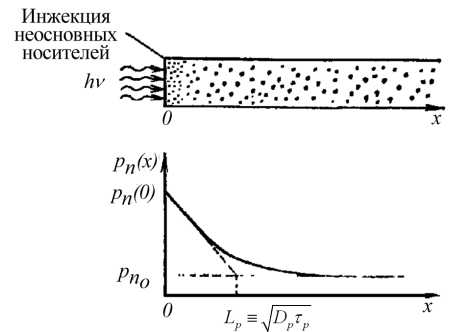
\includegraphics[]{8}
	\caption{Стационарная инжекция с одной стороны образца}
	\label{fig:figure7}
\end{figure}
% <img src="Время_жизни_2011_files/1240353c4f_3638373d38_2011-8.jpg" style="width:226pt;height:159pt;"/>

При помощи возбуждения светом и/или инжекции неосновных носителей заряда в полупроводник с помощью инжектирующих металлических контактов (или иным способом) можно также определить дрейфовую подвижность, коэффициент диффузии и другие параметры переноса. Примеры применения основных уравнений для решения данных задач можно найти в монографиях, приведенных в списке литературы.


\section{Экспериментальная часть}
Как показано в предыдущем разделе для измерения времени жизни и диффузионной длины неосновных носителей заряда необходимо создать неравновесное состояние электронно-дырочного газа в полупроводниковом кристалле. Сделать это проще всего при помощи облучения светом или инжектируя носители через контакты.

\subsection{Метод измерения времени жизни неосновных носителей заряда}

Для определения времени жизни используется метод модуляции проводимости, т.е. явления модуляции сопротивления области полупроводника вблизи точечного контакта металла с полупроводником при введении неосновных носителей из металла в полупроводник. Дело в том, что работы выхода электронов из металла и полупроводника в вакуум отличаются, поэтому при соединении этих материалов на границе раздела металл-полупроводник должен существовать энергетический барьер, величина которого равна разности соответствующих работ выхода. Носители вводятся в образец полупроводника через точечный контакт металл-полупроводник при помощи импульса тока, при этом они преодолевают энергетический барьер. Спустя некоторое время $\Delta t$ (время задержки), в течение которого происходят рекомбинация и диффузия носителей, введенных первым импульсом, прикладывается второй импульс, играющий роль измерительного. Падение напряжения на области полупроводника, примыкающей к точечному контакту наблюдается с помощью осциллографа по разности амплитуд импульсов.


На рисунке \ref{fig:figure8} показаны два импульса постоянного тока, поданных на образец в различные моменты времени, определяемые временем задержки второго импульса относительного первого. Уменьшение сопротивления, происходящее при введении носителей, приводит к уменьшению падения напряжения на точечном контакте. Так как ток через образец с помощью специальной радиотехнической схемы удерживается постоянным (рис.  \ref{fig:figure8}а), то форма импульса напряжения согласно закону Ома пропорциональна изменению сопротивления образца от времени. Уменьшение сопротивления образца обусловлено возрастанием концентрации носителей из-за их инжекции из металлического контакта. После прекращения первого импульса тока число неравновесных носителей постепенно уменьшается в результате рекомбинации, поэтому сопротивление области полупроводника вблизи точечного контакта начинает возвращаться к исходной величине, увеличиваясь со временем. При этом закон изменения сопротивления следует закону изменения числа носителей. Ввиду того, что при временах задержки меньших или сравнимых с временем жизни неосновных носителей заряда не все неосновные носители успевают рекомбинировать, импульс напряжения, соответствующий второму импульсу тока, будет несколько меньше по величине. Чем больше будет время задержки, тем меньше будет разница между первым и вторым импульсом напряжения. На рисунке \ref{fig:figure9} показана амплитуда напряжения второго импульса в зависимости от времени задержки. Огибающая кривая этих импульсов представляет собой закон возрастания сопротивления точечного контакта, следовательно, повторяет закон уменьшения числа неосновных носителей в результате рекомбинации.

\begin{figure}[H]
	\centering
	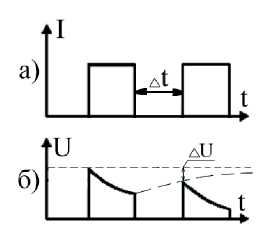
\includegraphics[]{9}
	\caption{Метод модуляции проводимости: а) импульсы тока, подаваемые на образец; б) изменение падения напряжения на образце. Величина $\Delta U$ зависит от времени задержки $\Delta t$}
	\label{fig:figure8}
\end{figure}
% <img src="Время_жизни_2011_files/1240353c4f_3638373d38_2011-9.jpg" style="width:132pt;height:111pt;"/>

\begin{figure}[H]
	\centering
	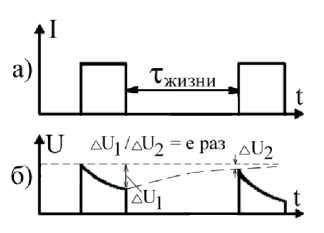
\includegraphics[]{10}
	\caption{Зависимость амплитуды второго импульса от времени задержки. В случае, когда время задержки равно времени жизни неосновных носителей заряда приращение амплитуды второго импульса составляет $e$ раз}
	\label{fig:figure9}
\end{figure}
% <img src="Время_жизни_2011_files/1240353c4f_3638373d38_2011-10.jpg" style="width:155pt;height:111pt;"/>



Этот закон описывается экспоненциальной функцией времени. Таким образом, зависимость разности амплитуд импульсов напряжения  $U_1-U_2$ от времени задержки, исключая окрестности точки $t = 0$, может быть представлена экспоненциальной функцией вида
\begin{gather}
	\label{eq17}
	U_{1}-U_{2} \sim e^{-t/\tau},
\end{gather}
где $\tau$ -- время жизни неосновных носителей заряда.

Соответственно зависимость $\ln(U_1-U_2)$ от $t$ графически изображается прямой линией, для которой обратное значение тангенса угла наклона равно по абсолютной величине времени жизни.

В данной работе используются точечные контакты, поэтому найдем падение напряжения на распределенном сопротивлении точечного контакта при пропускании через образец импульса постоянного тока $I$. Воспользуемся формулой
\begin{gather}
	\label{eq18}
	U=I R=\frac{\rho l}{S} I
\end{gather}
где $\rho$ -- удельное сопротивление, $l$ -- длина, $S$ -- сечение поверхности, через которую течет ток. 

Заметим, что формула \eqref{eq18} справедлива лишь для проводника с постоянным поперечным сечением $S$, когда линии тока параллельны друг другу. 
В нашем случае линии тока будут расходиться от острия контакта в радиальном направлении. Поэтому роль поперечного сечения будет играть поверхность полусферы переменного радиуса.
\begin{figure}[H]
	\centering
	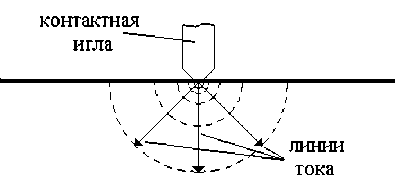
\includegraphics[]{11}
	\caption{Радиальное растекание тока от точечного контакта}
	\label{fig:figure10}
\end{figure}
% <img src="Время_жизни_2011_files/1240353c4f_3638373d38_2011-11.png" style="width:189pt;height:84pt;"/>

Ввиду этого необходимо произвести интегрирование по радиусу по всей области его изменения, то есть от $d$ до $\infty$ ($d$ -- радиус острия контакта). 

Тогда
\begin{gather}
	\label{eq19}
	U(t)=I \int_{d}^{\infty} \frac{\rho(t) \dd l}{2 \pi l^{2}}
\end{gather}

В формуле \eqref{eq19} $U$ не выражается явно как функция времени задержки $t$. Однако, зависимость $U$ от $t$ проявляется через удельное сопротивление, которое является функцией времени задержки.

Как было показано в разделе 1.3, концентрация неосновных носителей заряда изменяется со временем по экспоненциальному закону. Мы можем поэтому представить удельное сопротивление как сумму не зависящего от времени и экспоненциально убывающего слагаемых: 
\begin{gather}
	\label{eq20}
	\rho(t)=\rho_{0}+\rho_{1} e^{-\frac{t}{\tau}}
\end{gather}
где $\tau$ -0 время жизни неосновных носителей заряда.

Предположим, что время задержки между двумя импульсами тока равно $t$. Для этого случая найдем соответствующую разность импульсов напряжения. Очевидно, что для первого импульса тока время задержки следует считать равным бесконечности, так как для него $р = р_0$, что выполняется при $t\to\infty$. Поэтому
\begin{gather}
	\label{eq21}
	U_{1}-U_{2}=U(\infty)-U(t)=\frac{I}{2 \pi}\left(\int_{d}^{\infty} \frac{\rho_{0}}{l^{2}} d l-\int_{d}^{\infty} \frac{\rho_{0}-\rho_{1} e^{-\frac{t}{\tau}}}{l^{2}} d l\right)
\end{gather}
В результате получим уравнение вида
\begin{gather}
 	\label{eq22}
 	U_{1}-U_{2}=\left(\frac{I \rho_{1}}{2 \pi} \int_{d}^{\infty} \frac{d l}{l^{2}}\right) e^{-\frac{t}{\tau}},
 \end{gather}
 в котором множитель, стоящий в скобках, является постоянной величиной, не зависящей от времени задержки. Таким образом, разность импульсов напряжения со временем меняется по экспоненциальному закону \eqref{eq17}.

Необходимо отметить, что при рассмотрении метода мы пренебрегли поверхностной рекомбинацией. Учет этого явления сильно усложняет теорию, однако нетрудно создать экспериментальные условия, при которых упомянутое пренебрежение допустимо, уменьшение поверхностной рекомбинации по сравнению с объемной достигается путем подбора выгодной формы образца (малая удельная поверхность), протравливания образца (уменьшение числа поверхностных ловушек), освещение образца (освобождение захваченных ловушками носителей) и т.п.

Установка включает в себя блок генерации двух импульсов, позволяющий изменять время задержки между импульсами, держатель с образцом и осциллограф (рис.  \ref{fig:figure11}). Согласно методике, описанной выше, измеряя разность амплитуд импульсов в зависимости от задержки между ними можно определить время жизни неосновных носителей в образце. Для этого строится график зависимости логарифма этой разности от времени задержки. По котангенсу угла наклона определяется время жизни неосновных носителей.
\begin{figure}[H]
	\centering
	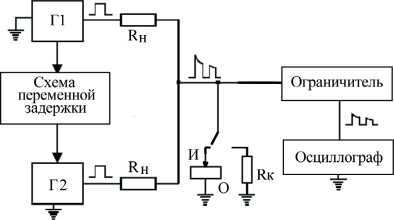
\includegraphics[]{12}
	\caption{Блок схема установки для измерения времени жизни:
И -- игла, О -- образец, $R_k$ -- калибровочное сопротивление, $R_h$ -- сопротивление нагрузки, Г1 и Г2 -- генераторы напряжения }
	\label{fig:figure11}
\end{figure}
% <img src="Время_жизни_2011_files/1240353c4f_3638373d38_2011-12.jpg" style="width:189pt;height:105pt;"/


\subsection{Метод измерения диффузионной длины неосновных носителей заряда}

Для определения диффузионной длины используют метод модуляции проводимости полупроводника при импульсном освещении, для чего применяют светодиод инфракрасного диапазона. Неравновесные носители, генерированные излучением светодиода, собираются с помощью вольфрамового зонда, служащего коллектором. Результирующий ток подается на сопротивление нагрузки, напряжение на котором регистрируется с помощью осциллографа.

\begin{figure}[H]
	\centering
	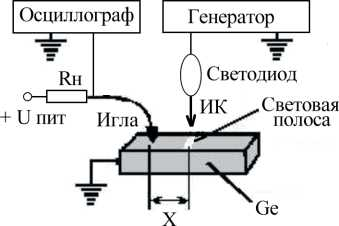
\includegraphics[]{13}
	\caption{Блок схема установки для измерения диффузионной длины неосновных носителей заряда}
	\label{fig:figure12}
\end{figure}

% <img src="Время_жизни_2011_files/1240353c4f_3638373d38_2011-13.jpg" style="width:162pt;height:108pt;"/>

Так как коллекторный ток прямо пропорционален концентрации неосновных носителей заряда вблизи точечного контакта, то можно считать, что падение напряжение на нагрузке прямо пропорционально концентрации дырок. Измеряя напряжение при различных расстояниях между коллектором и освещенной полосой можно определить диффузионную длину. По сути если световая полоса отодвинулась от коллектора на расстояние равное диффузионной длине, то амплитуда импульса напряжения изменилась в $е$ раз. Для более точного определения диффузионной длины строится график зависимости $\ln(U)$ от $x$. Котангенс угла наклона этой прямой определяет величину диффузионной длины.

Частота импульсов светодиода выбрана так, что во время импульса излучения в образце должно устанавливаться равномерное распределение неосновных носителей, а за время, когда образец не облучается, неосновные носители должны полностью рекомбинировать.

\subsection{Описание экспериментальной установки}

Экспериментальные установки для измерения времени жизни и диффузионной длины собраны в едином приборе, имеющем два режима работы (рис.  \ref{fig:figure13}). При измерении времени жизни вольфрамовая игла служит инжектором носителей. При измерении диффузионной длины генерация носителей осуществляется при помощи облучения, а игла служит коллектором.
\begin{figure}[H]
	\centering
	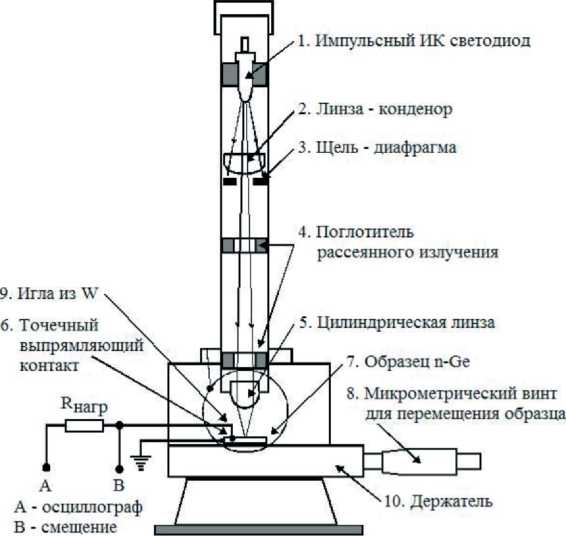
\includegraphics[]{14}
	\caption{Конструкция установки для генерации неравновесных носителей в образце. Установка работает в двух режимах: 1) инжекция (вброс) неосновных носителей заряда в полупроводниковый кристалл из металлического электрода - вольфрамовой иглы (светодиод выключен); 2) генерация неосновных носителей заряда в образце с помощью ПК излучения (игла играет роль коллектора носителей заряда)
}
	\label{fig:figure13}
\end{figure}
% <img src="Время_жизни_2011_files/1240353c4f_3638373d38_2011-14.jpg" style="width:271pt;height:257pt;"/>


Установка состоит из осветителя, в качестве которого используется импульсный светодиод инфракрасного диапазона \textbf{1}, оптической системы \textbf{2-5}, держателя \textbf{10}, в котором крепится образец \textbf{7} и осциллографа. Держатель представляет собой столик с кристаллодержателем, который может перемещаться в горизонтальном направлении. Отсчет продольного перемещения столика производится по микрометрическому винту \textbf{8}. К образцу прижимается вольфрамовый зонд \textbf{9}, служащий коллектором.

Схематический чертеж установки приведен на рисунке \ref{fig:figure13}. Излучение импульсного светодиода инфракрасного диапазона с помощью системы линз, изображенных на рисунке, фокусируется на образце n-Ge в линию шириной $\sim0.1$ мм, которая пересекает всю верхнюю грань образца и параллельна его торцам. Такая система освещения образца упрощает решение задачи диффузии неравновесных носителей, и на известном расстоянии от освещенного участка позволяет свести ее к одномерной задаче, рассмотренной выше.

\subsection{Задания}
\subsubsection{Диффузионная длина}
Определите диффузионную длину неосновных носителей тока, для этого нужно
\begin{itemize}
	\item включить на блоке тумблеры СЕТЬ и ОСВЕТИТЕЛЬ
	\item переключатель рода работ поставить в положение ДИФФ. ДЛИНА
	\item осциллограф: усиление У2: 50 мВ, развертка: 200 мкс
	\item синхронизация: ждущая (-), нажать кнопку Полоса Y2
\end{itemize}
Получив на экране осциллографа устойчивую картину импульса (при этом нужно крутить ручку УРОВЕНЬ синхронизации на осциллографе), ручкой СМЕЩЕНИЕ на блоке выставить ток 100 мкА.

Провести измерение амплитуды импульса (измеряя ее в мВ по масштабной сетке на экране осциллографа) в зависимости от расстояния х между световым пятном и щупом. Расстояния измеряются микрометрическим винтом, установленным на столике кристалл од ержателя. Измерения необходимо производить, начиная с максимальной амплитуды импульса до минимальной.

Построить график зависимости $\ln(U)$ как функции расстояния $x$. По наклону прямой определить диффузионную длину. Амплитуда импульса прямо пропорциональна концентрации неосновных носителей тока.

\subsubsection{Время жизни неосновных носителей тока}
Проведите измерение времени жизни неосновных носителей тока в n-Ge, для этого нужно
\begin{itemize}
	\item выключить ОСВЕТИТЕЛЬ
	\item переключатель поставить в положение КАЛИБРОВКА
	\item осциллограф: усиление У2: 50 мВ, развертка: 200 мкс
	\item осциллограф: усиление У2: 200 мВ, развертка: 5-10 мкс, синхронизация: ждущая (+)
\end{itemize}

Получить на экране осциллографа изображение двух импульсов.

Сравнять эти 2 импульса по величине ручкой КАЛИБРОВКА и установить амплитуду импульсов 200-250 мВ ручкой ОГРАНИЧЕНИЕ. Поставить переключатель в положение ВРЕМЯ ЖИЗНИ. Изменяя время задержки между импульсами от 0 до 100 мкс (при этом нужно крутить ручку ЗАДЕРЖКА на блоке), измерить зависимость разности амплитуд первого и второго импульсов от задержки по масштабной сетке на экране осциллографа.

Определить время жизни неосновных носителей тока.

\textit{Примечание. Нижние риски на неподвижной части микровинта, установленном на столике, соответствуют целым частям миллиметра, верхние риски -половинным долям мм (0.5мм). Риски на вращающейся части микровинта соответствуют сотым долям миллиметра.}

\subsection{Контрольные вопросы к лабораторной работе}

1. Что такое разрешенные и запрещенные зоны, уровень Ферми, вырожденные и невырожденные полупроводники, условие электронейтральности полупроводника, время жизни, диффузионная длина, подвижность, плотность состояний, концентрация носителей заряда (привести их характерные значения для Si, Ge, GaAs)?

2.    Что такое тип носителей заряда, собственные и примесные полупроводники? Привести примеры донорных и акцепторных примесей. Какова энергия ионизации примесных атомов? Как зависит подвижность от концентрации примесных атомов? Каков механизм рассеяния носителей заряда в полупроводниках?

3.    Как зависят от температуры ширина запрещенной зоны, уровень Ферми, подвижность, концентрация носителей заряда проводимость? Как связаны электропроводность, подвижность и концентрация носителей заряда? Методика измерения ширины запрещенной зоны. Как избежать влияния паразитной термоЭДС и контактных сопротивлений при измерениях?

\addcontentsline{toc}{section}{Список литературы}
\begin{thebibliography}{99}
\bibitem{land} Ландау Л.Д., Лифшиц Е.М. Теоретическая физика: т.5, Статистическая физика. - М.: Физматлит, 2005. - 616 с.

\bibitem{pp} Зи С.М. Физика полупроводниковых приборов. М.: Сов. Радио, 1984.

\bibitem{bb}   Бонч-Бруевич В.Л., Калашников С.Г. Физика полупроводников. 1977.

\bibitem{sh}    Шалимова К.В. Физика полупроводников. М.: 1982.
\end{thebibliography}

\end{document}


Измерение времени жизни и диффузионной длины неосновных носителей заряда в полупроводниках

Составители:

Ю. А. Битюрин, С. В. Оболенский, А. П. Чириманов, Н. В. Демарина, Е.В.Волкова, А.С.Пузанов

Подписано к печати Формат

Печать офсетная Уел. печ. л. тираж Бесплатно

Бумага оберточная Заказ

- 17 -

1

 Характерные длины волн оптического излучения составляют около 1 мкм, в то время как длина волны для электрона равна 10 нм.

Импульс и длина волны связаны соотношением p=hk = —, из чего

Л

получаем, что импульс фотона на 3 порядка меньше импульса электрона.

2

 В случае использования непрямозонных полупроводников для излучения света в них необходимо реализовать прямой переход не связанный с межзонным. Например, такой переход может быть реализован между различными уровнями атомов редкоземельных материалов, которые специально встраивают в решетку кремния для формирования светоизлучающих центров.
</body>
</html>
